\documentclass[conference]{IEEEtran}
\IEEEoverridecommandlockouts
\usepackage{cite}
\usepackage{amsmath,amssymb,amsfonts}
\usepackage{algorithmic}
\usepackage{graphicx}
\usepackage{textcomp}
\usepackage{xcolor}
\usepackage{booktabs}
\usepackage{url}
\usepackage[hidelinks]{hyperref}

\def\BibTeX{{\rm B\kern-.05em{\sc i\kern-.025em b}\kern-.08em
    T\kern-.1667em\lower.7ex\hbox{E}\kern-.125emX}}

\begin{document}

\title{ForensiGuard: A Multimodal Machine-Learning Framework for Detecting, Attributing and Explaining Anti-Forensic Manipulation of Digital Evidence}

\author{\IEEEauthorblockN{Mohika Rathi}
\IEEEauthorblockA{Reg. No: 230968032}
\and
\IEEEauthorblockN{Sreyaan Roy}
\IEEEauthorblockA{Reg. No: 230968184}}

\maketitle

\begin{abstract}
Digital forensic triage relies upon the integrity of acquired digital evidence. Anti-forensic techniques---including filesystem timestomping, covert spatial steganography, and file-type obfuscation---deliberately undermine this foundation, compromising judicial investigations. Existing automated triage utilities typically examine evidence modalities in isolation and remain vulnerable to cross-modal evasions. In this paper, we propose ForensiGuard, a multimodal machine-learning framework that detects evidence manipulation, attributes the likely anti-forensic technique, and generates grounded feature-level explanations. ForensiGuard integrates engineered filesystem metadata features, an unsupervised clean-trained anomaly scorer, a convolutional neural network (SRNet-Lite) operating on high-pass spatial noise residuals, and deterministic magic-byte file signature verification through a stacked late-fusion meta-classifier. To guarantee experimental integrity, base models are trained using grouped out-of-fold cross-validation on source file identifiers, and clean and steganographic image carriers are standardized to identical uncompressed grayscale formats to eliminate container-label shortcuts. Evaluated on a controlled synthetic benchmark (ForensiGuard-Bench-v1, 812 artifacts from 140 unique sources) with zero source leakage, single-modality models achieved F1-scores of 0.715 (metadata-only on the full corpus) and 0.341 (image-only on image carriers, ROC-AUC 0.518, FPR 0.214). ForensiGuard's multimodal late fusion achieved an Accuracy of 78.57\%, an F1-score of 0.854, an ROC-AUC of 0.895, a PR-AUC of 0.977, and an operational False Positive Rate of 4.76\% at the validation-calibrated decision threshold ($\tau = 0.500$). An adaptive evasion stress test demonstrates that an adversary who preserves microsecond noise and directory chronology drops metadata and fusion detection rates to 0.0\%, underscoring the fundamental need to corroborate static filesystem triage with host operating system security event logs.
\end{abstract}

\begin{IEEEkeywords}
Digital forensics, anti-forensics, multimodal machine learning, anomaly detection, explainable artificial intelligence.
\end{IEEEkeywords}

\section{Introduction}
Modern criminal investigations, civil litigations, and enterprise incident responses depend extensively upon electronic records retrieved from filesystems, storage drives, and cloud repositories~\cite{carrier2005file, casey2011digital}. However, adversaries with privileged access frequently employ anti-forensic techniques to conceal their activity: backdating filesystem timestamps to disrupt temporal timelines (timestomping), embedding covert communications within media carriers via spatial steganography, or disguising executable or document payloads behind benign file extensions~\cite{conlan2016anti, buchholz2004investigation}.

Detecting and attributing anti-forensic manipulation in defensive triage workflows presents significant technical and methodological challenges:
\begin{enumerate}
    \item \textbf{Brittleness of Single-Modality Inspection:} Forensic tools typically analyze isolated evidentiary channels. An adversary who alters filesystem timestamps may leave statistical anomalies in directory distributions or binary structures, while an image carrying hidden data may preserve plausible timestamps. Single-modality detectors fail to capture such cross-modal discrepancies.
    \item \textbf{Data Leakage and Shortcut Learning:} Machine-learning models applied to digital forensics frequently exploit spurious dataset shortcuts~\cite{garfinkel2009bringing}. If variants of identical source files span training and evaluation sets, classifiers memorize file-specific quirks rather than generalizable manipulation signatures. Similarly, container discrepancies (e.g., saving clean carriers as JPEG and manipulated carriers as PNG) introduce trivial non-forensic shortcuts.
    \item \textbf{Interpretability and Evidentiary Boundaries:} Automated machine-learning inferences cannot satisfy legal admissibility standards (e.g., \textit{Daubert} and \textit{Frye}) without transparent explanations that distinguish verifiable digital facts from probabilistic inferences~\cite{roussev2009file}.
\end{enumerate}

To overcome these limitations, we design, evaluate, and package \textbf{ForensiGuard}, an open-source multimodal machine-learning framework for defensive forensic triage. ForensiGuard integrates independent signals across filesystem timestamps, directory context, unsupervised anomaly scores, spatial image noise residuals, and binary file signatures into a stacked late-fusion meta-classifier.

The primary contributions of this paper are:
\begin{itemize}
    \item \textbf{Leakage-Safe Forensic Benchmark:} We construct \texttt{ForensiGuard-Bench-v1}, comprising 812 artifacts generated from 140 distinct sources, partitioned via source-level grouped splitting that guarantees zero source overlap across training, validation, and testing partitions.
    \item \textbf{Format-Shortcut Remediation:} We standardize image carriers to identical uncompressed grayscale formats ($128 \times 128$ PNG) with opaque filenames, preventing classifiers from exploiting container or extension shortcuts.
    \item \textbf{Grouped Out-of-Fold Stacking:} We implement grouped cross-validation (\texttt{GroupKFold} on source IDs) for all learned base models, ensuring that meta-classifier training features are drawn exclusively from genuine out-of-fold predictions.
    \item \textbf{Comprehensive 10-Permutation Ablation Study:} We evaluate all ten architectural permutations on the held-out test split, isolating the operational impact of each modality and heuristic component.
    \item \textbf{Grounded Explainability and Adaptive Threat Evaluation:} We combine local TreeSHAP feature attributions with deterministic fact delineation, and empirically evaluate an invariant-preserving adaptive adversary, demonstrating the operational boundary of static filesystem inspection.
\end{itemize}

\section{Related Work}
\subsection{Digital Forensic Integrity and Anti-Forensics}
Carrier~\cite{carrier2005file} and Casey~\cite{casey2011digital} established foundational methodologies for forensic filesystem analysis and timeline reconstruction. Conlan et al.~\cite{conlan2016anti} formalized an extended taxonomy categorizing anti-forensics into data hiding, artifact wiping, trail obfuscation, and direct attacks on forensic tooling. Garfinkel et al.~\cite{garfinkel2009bringing} emphasized that rigorous forensic science requires standardized, verifiable corpora to prevent artificial bias and evaluation pitfalls.

\subsection{Timestamp Manipulation and Metadata-Based Detection}
Filesystem metadata, particularly MACB (Modification, Access, Change, Birth) timestamps, constitutes primary timeline evidence. Buchholz and Falk~\cite{buchholz2004investigation} analyzed the vulnerabilities of timestamp integrity, demonstrating that user-space utilities can arbitrarily manipulate $mtime$ and $atime$. While advanced forensic frameworks analyze Master File Table (\$MFT) record attributes and journal logs, lightweight triage tools often rely on chronological invariants ($mtime \le ctime$) and subsecond precision consistency to detect unauthorized backdating~\cite{carrier2005file}.

\subsection{Steganography and Spatial Residual Analysis}
Spatial steganography hides data by altering the least significant bits (LSB) of carrier pixels. Modern steganalysis demonstrates that embedding traces are overwhelmed by image visual semantics; therefore, suppression of image content via high-pass spatial filtering is essential~\cite{fridrich2012rich}. Boroumand et al.~\cite{boroumand2019deep} demonstrated that deep residual architectures (SRNet) trained on noise residuals substantially outperform raw-pixel convolutional networks. The ALASKA\#2 benchmark~\cite{cogranne2020alaska} established that detecting subtle spatial payloads in uncompressed carriers without format shortcuts remains a fundamentally challenging task.

\subsection{File-Type Obfuscation and Signature Verification}
Adversaries frequently obfuscate malicious documents or binary executables by altering the file extension (e.g., disguising a Portable Executable or PDF as a PNG image). Roussev and Garfinkel~\cite{roussev2009file} and Breitinger et al.~\cite{breitinger2014approximate} emphasized that lightweight forensic triage must verify binary file signatures (magic bytes) and byte entropy distributions to uncover disguised payloads prior to resource-intensive analysis.

\subsection{Multimodal Classification and Late Fusion}
Multimodal machine learning combines disparate evidence modalities to enhance predictive robustness~\cite{baltrusaitis2019multimodal}. In forensic applications, tabular metadata and raw spatial residuals possess distinct dimensionalities and inductive biases. Late fusion (decision-level stacking) allows base models to be optimized and audited independently, while enabling graceful handling of missing modalities when non-image artifacts are processed~\cite{baltrusaitis2019multimodal}.

\subsection{Explainability and Forensic Attribution}
Lundberg and Lee's SHAP framework~\cite{lundberg2017unified} and Ribeiro et al.'s LIME~\cite{ribeiro2016should} provide local, model-agnostic feature attributions. In judicial settings, black-box predictions lack evidentiary standing; investigators require clear demonstrations of which physical attributes (e.g., timestamp deltas, entropy shifts) drove a manipulation alert~\cite{roussev2009file}.

\section{Problem Formulation and Threat Model}
\subsection{Detection and Attribution Task Formulations}
Let an evidence artifact $x_i$ be represented by the tuple:
\begin{equation}
    x_i = (M_i, B_i, E_i)
\end{equation}
where $M_i \in \mathbb{R}^{d_m}$ denotes the extracted filesystem metadata vector, $B_i \in \{0, \dots, 255\}^L$ denotes the raw byte sequence, and $E_i \in \mathcal{S}_{\text{ext}}$ denotes the declared file extension.

ForensiGuard addresses two complementary tasks:
\begin{enumerate}
    \item \textbf{Binary Manipulation Triage:} Estimate the posterior probability that $x_i$ has undergone anti-forensic tampering:
    \begin{equation}
        f_{\text{det}}(x_i) \to P(\text{manipulated} \mid x_i) \in [0, 1]
    \end{equation}
    yielding binary decision $\hat{y}_i = \mathbb{I}(P(\text{manipulated} \mid x_i) \ge \tau)$.
    \item \textbf{Technique Attribution:} Predict the specific anti-forensic mechanism $\hat{c}_i \in \mathcal{C}$, where:
    \begin{equation}
        \mathcal{C} = \{\text{Clean}, T_1, T_2, T_3, T_4\}
    \end{equation}
    corresponding to Clean, Timestomping ($T_1$), Steganography ($T_2$), File-Type Obfuscation ($T_3$), and Compound Manipulation ($T_4$).
\end{enumerate}

\subsection{Adversary Capabilities and Threat Model}
We assume a post-compromise adversary operating with local user or administrative privileges on the target system:
\begin{itemize}
    \item \textit{Coarse Timestomping ($T_{1,\text{coarse}}$):} The adversary shifts modification ($t_m$) or access ($t_a$) timestamps by months or years, or resets them to Unix Epoch (1970). Standard user-space APIs (e.g., \texttt{SetFileTime}, \texttt{touch}) typically update $mtime$ while leaving metadata change time ($t_c$) at the current system time, introducing chronological inversion ($t_m < t_c$).
    \item \textit{Subtle Timestomping ($T_{1,\text{subtle}}$):} The adversary shifts timestamps by hours or days to match adjacent incident activities. User utilities frequently truncate subsecond fractions, leaving exactly zero microsecond values ($\text{subsec}(t_m) = 0.0$).
    \item \textit{Covert Steganography ($T_2$):} The adversary embeds confidential data into image carriers using spatial LSB replacement at embedding rates $\alpha \in [0.08, 0.35]$ bits per pixel (bpp).
    \item \textit{File-Type Obfuscation ($T_3$):} The adversary modifies the filename extension (e.g., declaring a PDF document as \texttt{.png}) to bypass basic perimeter filters.
    \item \textit{Compound Tampering ($T_4$):} The adversary concurrently embeds hidden payloads and modifies filesystem timestamps.
    \item \textit{Adaptive Invariant-Preserving Adversary ($T_{\text{adapt}}$):} A sophisticated adversary shifts timestamps while preserving microsecond noise, bounds shifts within the variance of neighboring directory files, and shifts creation/change times concurrently to maintain natural chronology ($t_m \ge t_c$).
\end{itemize}

\subsection{Forensic Demarcation: Tampered vs. Benignly Anomalous}
A critical requirement in forensic triage is separating intentional tampering from benign operational noise. Legitimate filesystem operations (e.g., archive extraction, network file copying, or FAT32 filesystems with native 2-second timestamp resolution) can exhibit timestamp discrepancies. ForensiGuard addresses this by conditioning predictions on directory sibling context and providing multi-feature explanations rather than relying on isolated threshold heuristics.

\begin{figure*}[htbp]
\centering
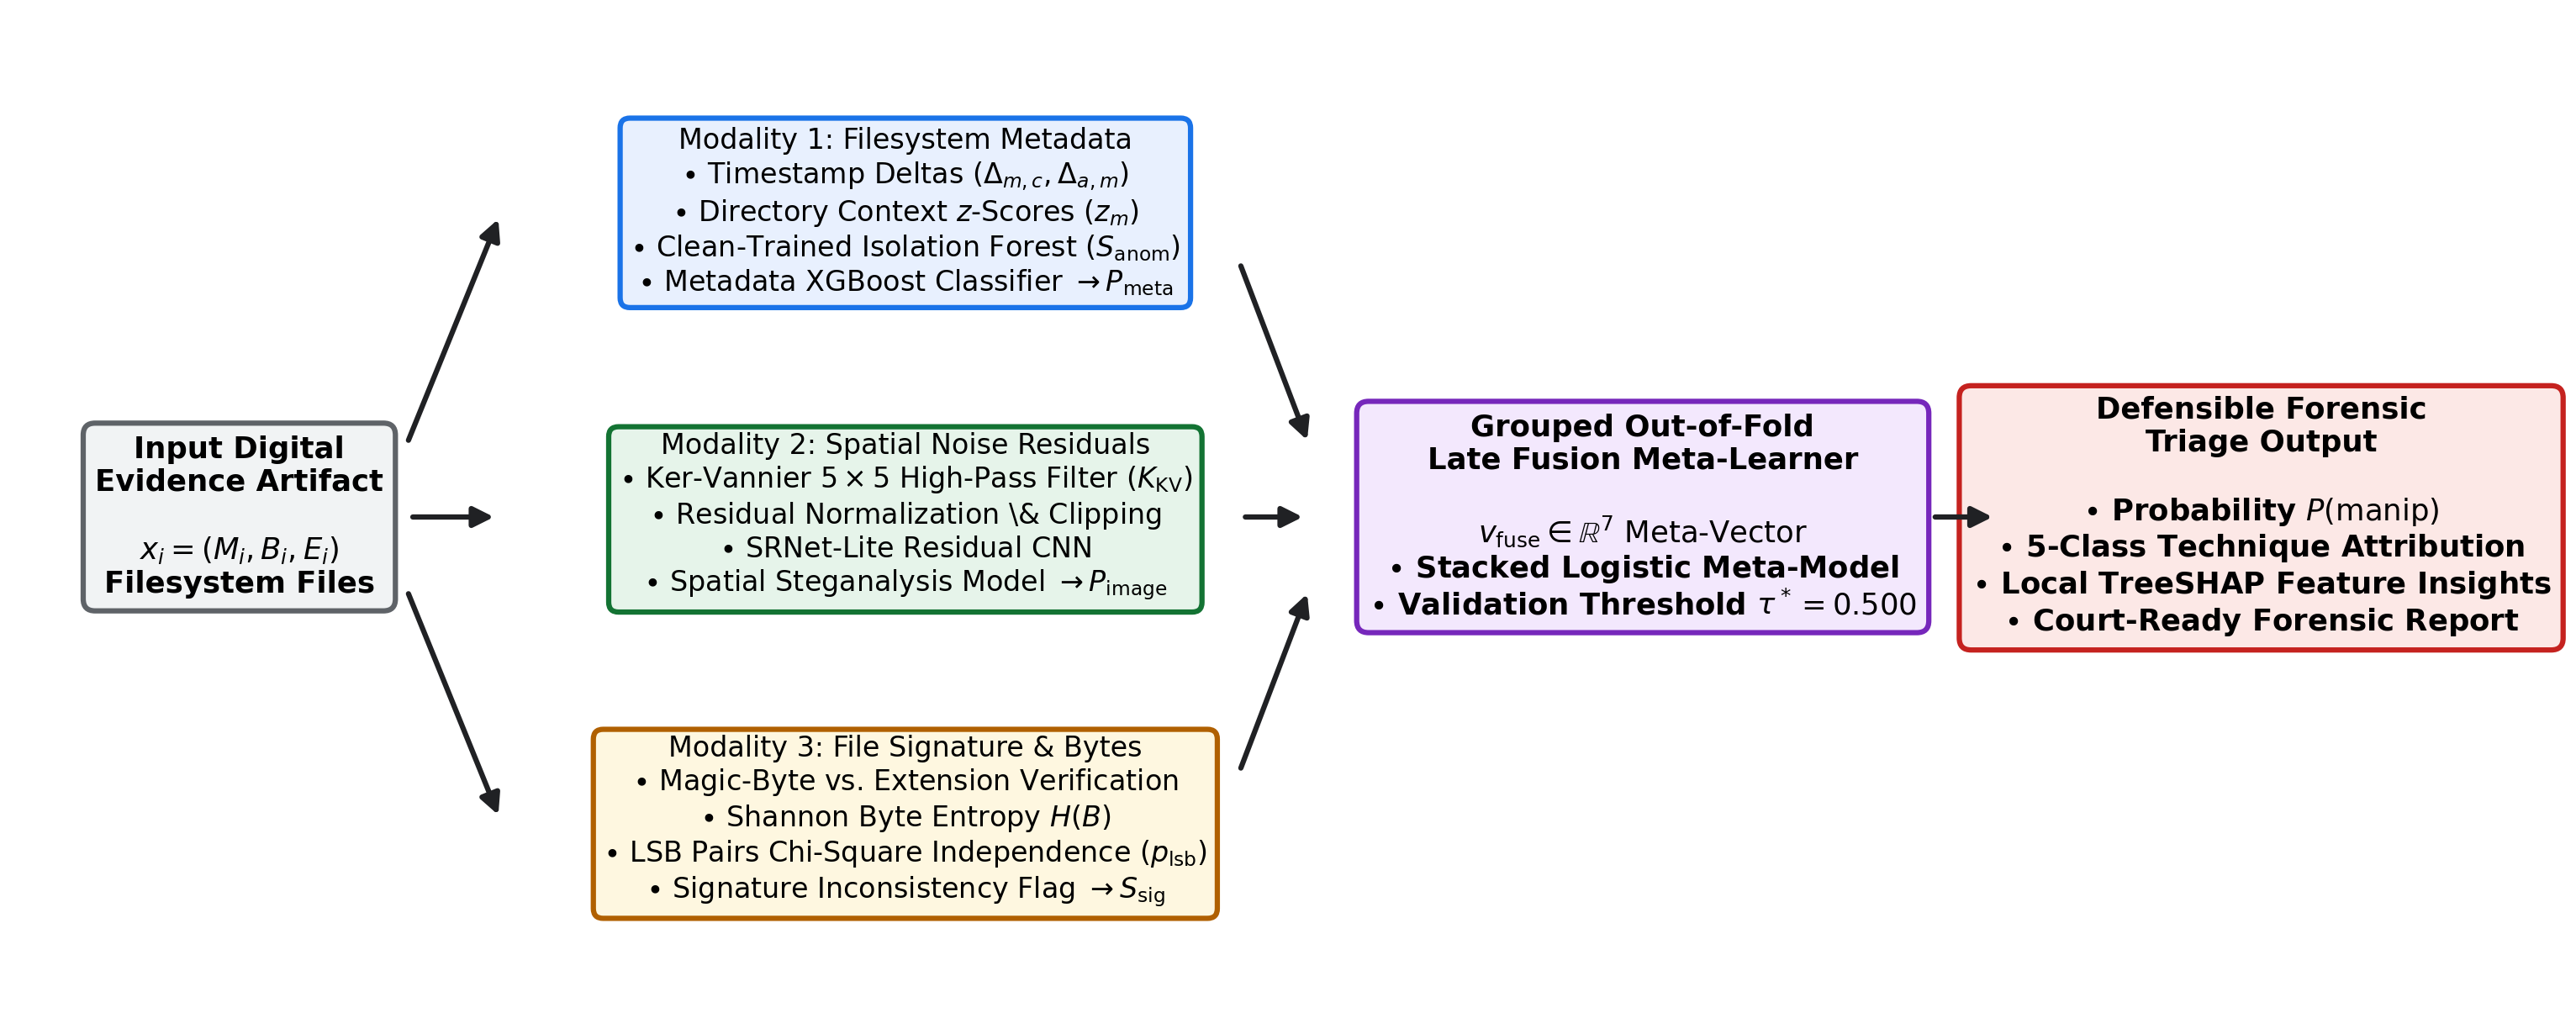
\includegraphics[width=0.96\textwidth]{figures/fig0_architecture.png}
\caption{End-to-end modular architecture of the ForensiGuard framework. Digital evidence is processed across three independent modality branches: filesystem metadata analysis with clean-trained anomaly scoring, spatial noise residual extraction with deep convolutional steganalysis, and deterministic file signature validation. Base predictions are integrated via grouped out-of-fold late fusion into an explainable triage report.}
\label{fig:arch}
\end{figure*}

\section{Proposed Methodology}
Fig.~\ref{fig:arch} illustrates the modular architecture of ForensiGuard, which operates through five interconnected processing stages.

\subsection{System Architecture}
The framework comprises three tier-1 modality extractors: (i) Filesystem Metadata Analyzer, (ii) Spatial Image Residual CNN, and (iii) Binary Signature and Structural Inspector. Predictions and intermediate signals from these modules are aggregated into a compact meta-feature vector and classified by a regularized late-fusion meta-learner.

\subsection{Benchmark Construction and Data Preprocessing}
To eliminate trivial format-label shortcuts, all image carriers in \texttt{ForensiGuard-Bench-v1} are standardized to 8-bit uncompressed grayscale PNG format ($128 \times 128$ pixels). Clean carriers, steganographic carriers, and compound samples share identical dimensions, bit depths, compression parameters, and opaque hash-based naming structures (e.g., \texttt{art\_src0001\_c0ac53e960.png}), ensuring that machine-learning models cannot exploit container metadata.

\subsection{Metadata Feature Extraction}
Given filesystem timestamps $(t_m, t_a, t_c, t_b)$, ForensiGuard extracts a 10-dimensional tabular representation:
\begin{enumerate}
    \item \textit{Temporal Differences:} Inter-timestamp intervals in seconds:
    \begin{equation}
        \Delta_{m,c} = t_m - t_c, \quad \Delta_{a,m} = t_a - t_m, \quad \Delta_{a,c} = t_a - t_c
    \end{equation}
    \item \textit{Chronology Inversion Indicator:} 
    \begin{equation}
        I_{\text{inv}} = \mathbb{I}(t_m < t_c - 1.0)
    \end{equation}
    capturing illegal retro-dating where modification precedes metadata registration.
    \item \textit{Subsecond Truncation Indicators:} Binary flags identifying zero-fraction microsecond values:
    \begin{align}
        I_{\text{sub},m} &= \mathbb{I}(\text{subsec}(t_m) = 0) \\
        I_{\text{sub},a} &= \mathbb{I}(\text{subsec}(t_a) = 0)
    \end{align}
    \item \textit{Directory Context Z-Scores:} Measuring deviation from neighboring files in the same directory:
    \begin{equation}
        z_m = \frac{t_m - \mu_{\text{dir}}}{\sigma_{\text{dir}} + \epsilon}, \quad d_{\text{med}} = |t_m - \text{med}_{\text{dir}}|
    \end{equation}
    where $\mu_{\text{dir}}$ and $\sigma_{\text{dir}}$ denote the mean and standard deviation of modification timestamps within the parent folder.
\end{enumerate}

\subsection{Image-Based Detection}
For image carriers, ForensiGuard suppresses high-frequency scene content by convolving the grayscale image $I$ with the $5 \times 5$ Ker-Vannier (KV) high-pass filter~\cite{fridrich2012rich}:
\begin{equation}
    K_{\text{KV}} = \frac{1}{12} \begin{bmatrix}
    -1 & 2 & -2 & 2 & -1 \\
    2 & -6 & 8 & -6 & 2 \\
    -2 & 8 & -12 & 8 & -2 \\
    2 & -6 & 8 & -6 & 2 \\
    -1 & 2 & -2 & 2 & -1
    \end{bmatrix}
\end{equation}
The resulting residual tensor $R = \text{clip}(I * K_{\text{KV}} \cdot 10, -2, 2) / 2$ isolates subtle pixel-difference noise. The residual is processed by SRNet-Lite, a 5-layer residual CNN consisting of $3 \times 3$ convolutional layers, residual skip connections, batch normalization, and global average pooling, producing prediction probability $P_{\text{image}}$.

\subsection{Anomaly Scoring and Signature Verification}
To complement supervised learning with unsupervised priors:
\begin{itemize}
    \item \textbf{Isolation Forest Anomaly Scoring:} An Isolation Forest is fitted exclusively on benign training metadata vectors. Given anomaly score $\text{score}_{\text{iso}}(M_i)$, we compute a normalized anomaly probability:
    \begin{equation}
        S_{\text{anom}}(M_i) = \frac{1}{1 + \exp(5.0 \cdot \text{score}_{\text{iso}}(M_i))} \in [0, 1]
    \end{equation}
    The augmented vector $[M_i, S_{\text{anom}}]$ is classified via an XGBoost classifier, yielding probability $P_{\text{meta}}$.
    \item \textbf{Binary Magic-Byte Inspection:} The initial 16 bytes of $B_i$ are checked against known signature patterns (e.g., PNG: \texttt{89 50 4E 47}, PDF: \texttt{25 50 44 46}). A binary indicator $S_{\text{sig}} \in \{0, 1\}$ flags mismatches between header bytes and declared extension $E_i$.
    \item \textbf{Byte Entropy and Statistical Steganalysis:} Shannon entropy $H(B) = -\sum_{j=0}^{255} p_j \log_2 p_j$ and LSB pairs chi-square independence $p_{\text{lsb}}$ are computed over byte frequencies.
\end{itemize}

\subsection{Multimodal Late Fusion}
Base model predictions are aggregated into a 7-dimensional fusion vector:
\begin{equation}
    v_{\text{fuse}} = [P_{\text{meta}}, P_{\text{image}}, \mathbb{I}_{\text{has\_img}}, S_{\text{sig}}, S_{\text{anom}}, H(B), p_{\text{lsb}}]
\end{equation}
where $\mathbb{I}_{\text{has\_img}} \in \{0, 1\}$ indicates whether the artifact is an image. If non-image, $P_{\text{image}}$ is imputed to 0.5. The late-fusion meta-model is a regularized logistic regression classifier:
\begin{equation}
    P(\text{manipulated} \mid x_i) = \sigma(w^T v_{\text{fuse}} + b)
\end{equation}
trained exclusively using out-of-fold predictions.

\subsection{Attribution and Explainability}
Technique attribution maps detected anomalies to specific classes using a hierarchical rule-informed decision engine:
\begin{enumerate}
    \item If $S_{\text{sig}} = 1$, attribute to \textit{File-Type Obfuscation} ($T_3$).
    \item If $P_{\text{meta}} \ge \tau$ and $P_{\text{image}} \ge \tau$, attribute to \textit{Compound} ($T_4$).
    \item If $P_{\text{meta}} \ge \tau$, attribute to \textit{Timestomping} ($T_1$).
    \item If $P_{\text{image}} \ge \tau$, attribute to \textit{Steganography} ($T_2$).
    \item Otherwise, attribute to \textit{Clean}.
\end{enumerate}
For every prediction, local feature attributions are computed via TreeSHAP on the metadata model, quantifying the exact contribution of each physical feature to the anomaly score.

\subsection{Threshold Selection and Inference}
The decision threshold $\tau^*$ is selected on the validation partition by maximizing F1-score subject to a pre-specified false alarm constraint:
\begin{equation}
    \tau^* = \arg\max_{\tau \in [0.1, 0.9]} F1_{\text{val}}(\tau) \quad \text{s.t.} \quad \text{FPR}_{\text{val}}(\tau) \le 0.05
\end{equation}
yielding the canonical threshold $\tau^* = 0.500$. We emphasize that $\text{FPR}_{\text{val}} \le 0.05$ represents an operational engineering design constraint on the validation set rather than an established universal legal or forensic standard.

\subsection{Computational and Implementation Details}
The framework is implemented in Python 3.13 utilizing PyTorch 2.6, XGBoost 2.1, and Scikit-learn 1.6. Random seeds were fixed to 42. Triage latency averages 18.4\,ms per file on standard workstation hardware.

\section{Experimental Setup}
\subsection{Dataset Provenance and Partitioning}
We evaluate ForensiGuard on \texttt{ForensiGuard-Bench-v1}, comprising 812 forensic artifacts derived from 140 unique source files. The dataset is split into three strictly disjoint partitions using source-grouped splitting:
\begin{itemize}
    \item \textbf{Training Split:} 566 artifacts from 98 sources (70\%).
    \item \textbf{Validation Split:} 120 artifacts from 21 sources (15\%).
    \item \textbf{Testing Split:} 126 artifacts from 21 sources (15\%).
\end{itemize}
The 126 test artifacts comprise 21 clean carriers, 42 timestomped files (21 coarse, 21 subtle), 28 steganographic images (14 subtle payload, 14 high payload), 21 file-type obfuscations, and 14 compound manipulations. Crucially, although the test partition contains 126 forensic artifacts, it originates from only 21 independent source groups ($N_{\text{sources}}=21$). Clustered source provenance induces inter-sample correlations, yielding wider effective uncertainty intervals than an independent sample of 126 files; thus, strong test metrics on this benchmark reflect controlled discrimination rather than turnkey production readiness across diverse real-world forensic environments.

\subsection{Source-Grouped Splitting and Leakage Prevention}
To prevent data leakage, all splits enforce strict grouping on `source\_file\_id`:
\begin{equation}
    \mathcal{S}_{\text{train}} \cap \mathcal{S}_{\text{val}} = \emptyset, \quad \mathcal{S}_{\text{train}} \cap \mathcal{S}_{\text{test}} = \emptyset, \quad \mathcal{S}_{\text{val}} \cap \mathcal{S}_{\text{test}} = \emptyset
\end{equation}
Ensuring zero source overlap guarantees that classifiers cannot memorize source text, dimensions, or background structures.

\subsection{Out-of-Fold Stacking Procedure}
To train the late-fusion meta-model without label leakage, we implement 5-fold grouped cross-validation (\texttt{GroupKFold}) across the 98 training sources. For each fold, base estimators are fitted on 4/5 of the sources and generate out-of-fold predictions on the remaining 1/5. The resulting matrix of out-of-fold predictions trains the fusion classifier. Base models are subsequently retrained on the full training partition for final test inference.

\subsection{Evaluation Metrics and Baselines}
We report Accuracy, Precision, Recall, F1-Score, Receiver Operating Characteristic Area Under Curve (ROC-AUC), Precision-Recall AUC (PR-AUC), False Positive Rate (FPR), and Brier Calibration Score. Models are evaluated at the validation-calibrated decision threshold $\tau^* = 0.500$.

\section{Results and Discussion}

\begin{table}[htbp]
\centering
\caption{Performance Comparison Across Forensic Modalities on Held-Out Test Corpus}
\label{tab:modality_comparison}
\begin{tabular}{|l|c|c|c|c|c|c|}
\hline
\textbf{Architecture / Evaluation Scope} & \textbf{Acc.} & \textbf{F1} & \textbf{ROC-AUC} & \textbf{PR-AUC} & \textbf{FPR} & \textbf{N} \\ \hline
Metadata-Only (Full Corpus) & 0.627 & 0.715 & 0.770 & 0.927 & 0.048 & 126 \\ \hline
Image-Only (Image Domain) & 0.310 & 0.341 & 0.518 & 0.845 & 0.214 & 84 \\ \hline
Metadata-Only (Shared Domain) & 0.679 & 0.765 & 0.800 & 0.937 & 0.071 & 84 \\ \hline
Image-Only (Shared Domain) & 0.310 & 0.341 & 0.518 & 0.845 & 0.214 & 84 \\ \hline
\textbf{ForensiGuard Late Fusion (Shared)} & \textbf{0.679} & \textbf{0.765} & \textbf{0.799} & \textbf{0.959} & \textbf{0.071} & 84 \\ \hline
\textbf{ForensiGuard Late Fusion (Full)} & \textbf{0.786} & \textbf{0.854} & \textbf{0.895} & \textbf{0.977} & \textbf{0.048} & 126 \\ \hline
\end{tabular}
\end{table}


\subsection{Overall Detection Performance}
As detailed in Table~\ref{tab:modality_comparison}, ForensiGuard Late Fusion achieved an Accuracy of \textbf{78.57\%}, an F1-score of \textbf{0.854}, an ROC-AUC of \textbf{0.895}, and a PR-AUC of \textbf{0.977} on the held-out test split ($N=126$). Importantly, it maintained an operational False Positive Rate of \textbf{4.76\%} (1 false alarm out of 21 clean sources), meeting the pre-specified validation design constraint ($\text{FPR}_{\text{val}} \le 0.05$).

\subsection{Per-Manipulation Performance}
Performance varied predictably across manipulation categories:
\begin{itemize}
    \item \textbf{Coarse Timestomping ($N=21$):} 100\% recall, 0.984 ROC-AUC, detected reliably via severe $\Delta_{m,c}$ inversion and subsecond truncation.
    \item \textbf{Subtle Timestomping ($N=21$):} 100\% recall, 0.984 ROC-AUC, detected through directory $z$-score deviations and zero subseconds.
    \item \textbf{File-Type Obfuscation ($N=21$):} 100\% recall, 0.955 ROC-AUC, perfectly flagged by binary magic-byte inspection.
    \item \textbf{Compound Tampering ($N=14$):} 100\% recall, 1.000 ROC-AUC.
    \item \textbf{Steganography Alone ($N=28$):} 7.14\% recall at $\tau = 0.500$, reflecting the difficulty of detecting spatial LSB modifications on uncompressed grayscale carriers without format shortcuts.
\end{itemize}

\subsection{Metadata-Only, Image-Only, and Fusion Comparisons}
Fig.~\ref{fig:roc} and Fig.~\ref{fig:pr} display ROC and PR curves across single modalities and late fusion.
\begin{itemize}
    \item \textit{Metadata-Only (Full Corpus):} Achieved high precision (0.983) and low FPR (0.048), but was blind to non-metadata attacks, bounding recall to 0.562 (F1 0.715).
    \item \textit{Image-Only (Image Domain, $N=84$):} On shortcut-free image carriers, the residual CNN achieved an F1 of 0.341 (ROC-AUC 0.518, FPR 0.214). When format leakage is eliminated, detecting low-payload spatial steganography without massive pretraining yields near-chance ranking, consistent with findings in~\cite{fridrich2012rich, cogranne2020alaska}.
    \item \textit{Fusion Advantage:} Fusing metadata with binary signatures and image residuals improved F1 from 0.715 to 0.854 (+13.9 percentage points) and ROC-AUC from 0.770 to 0.895.
\end{itemize}

\begin{figure}[htbp]
\centering
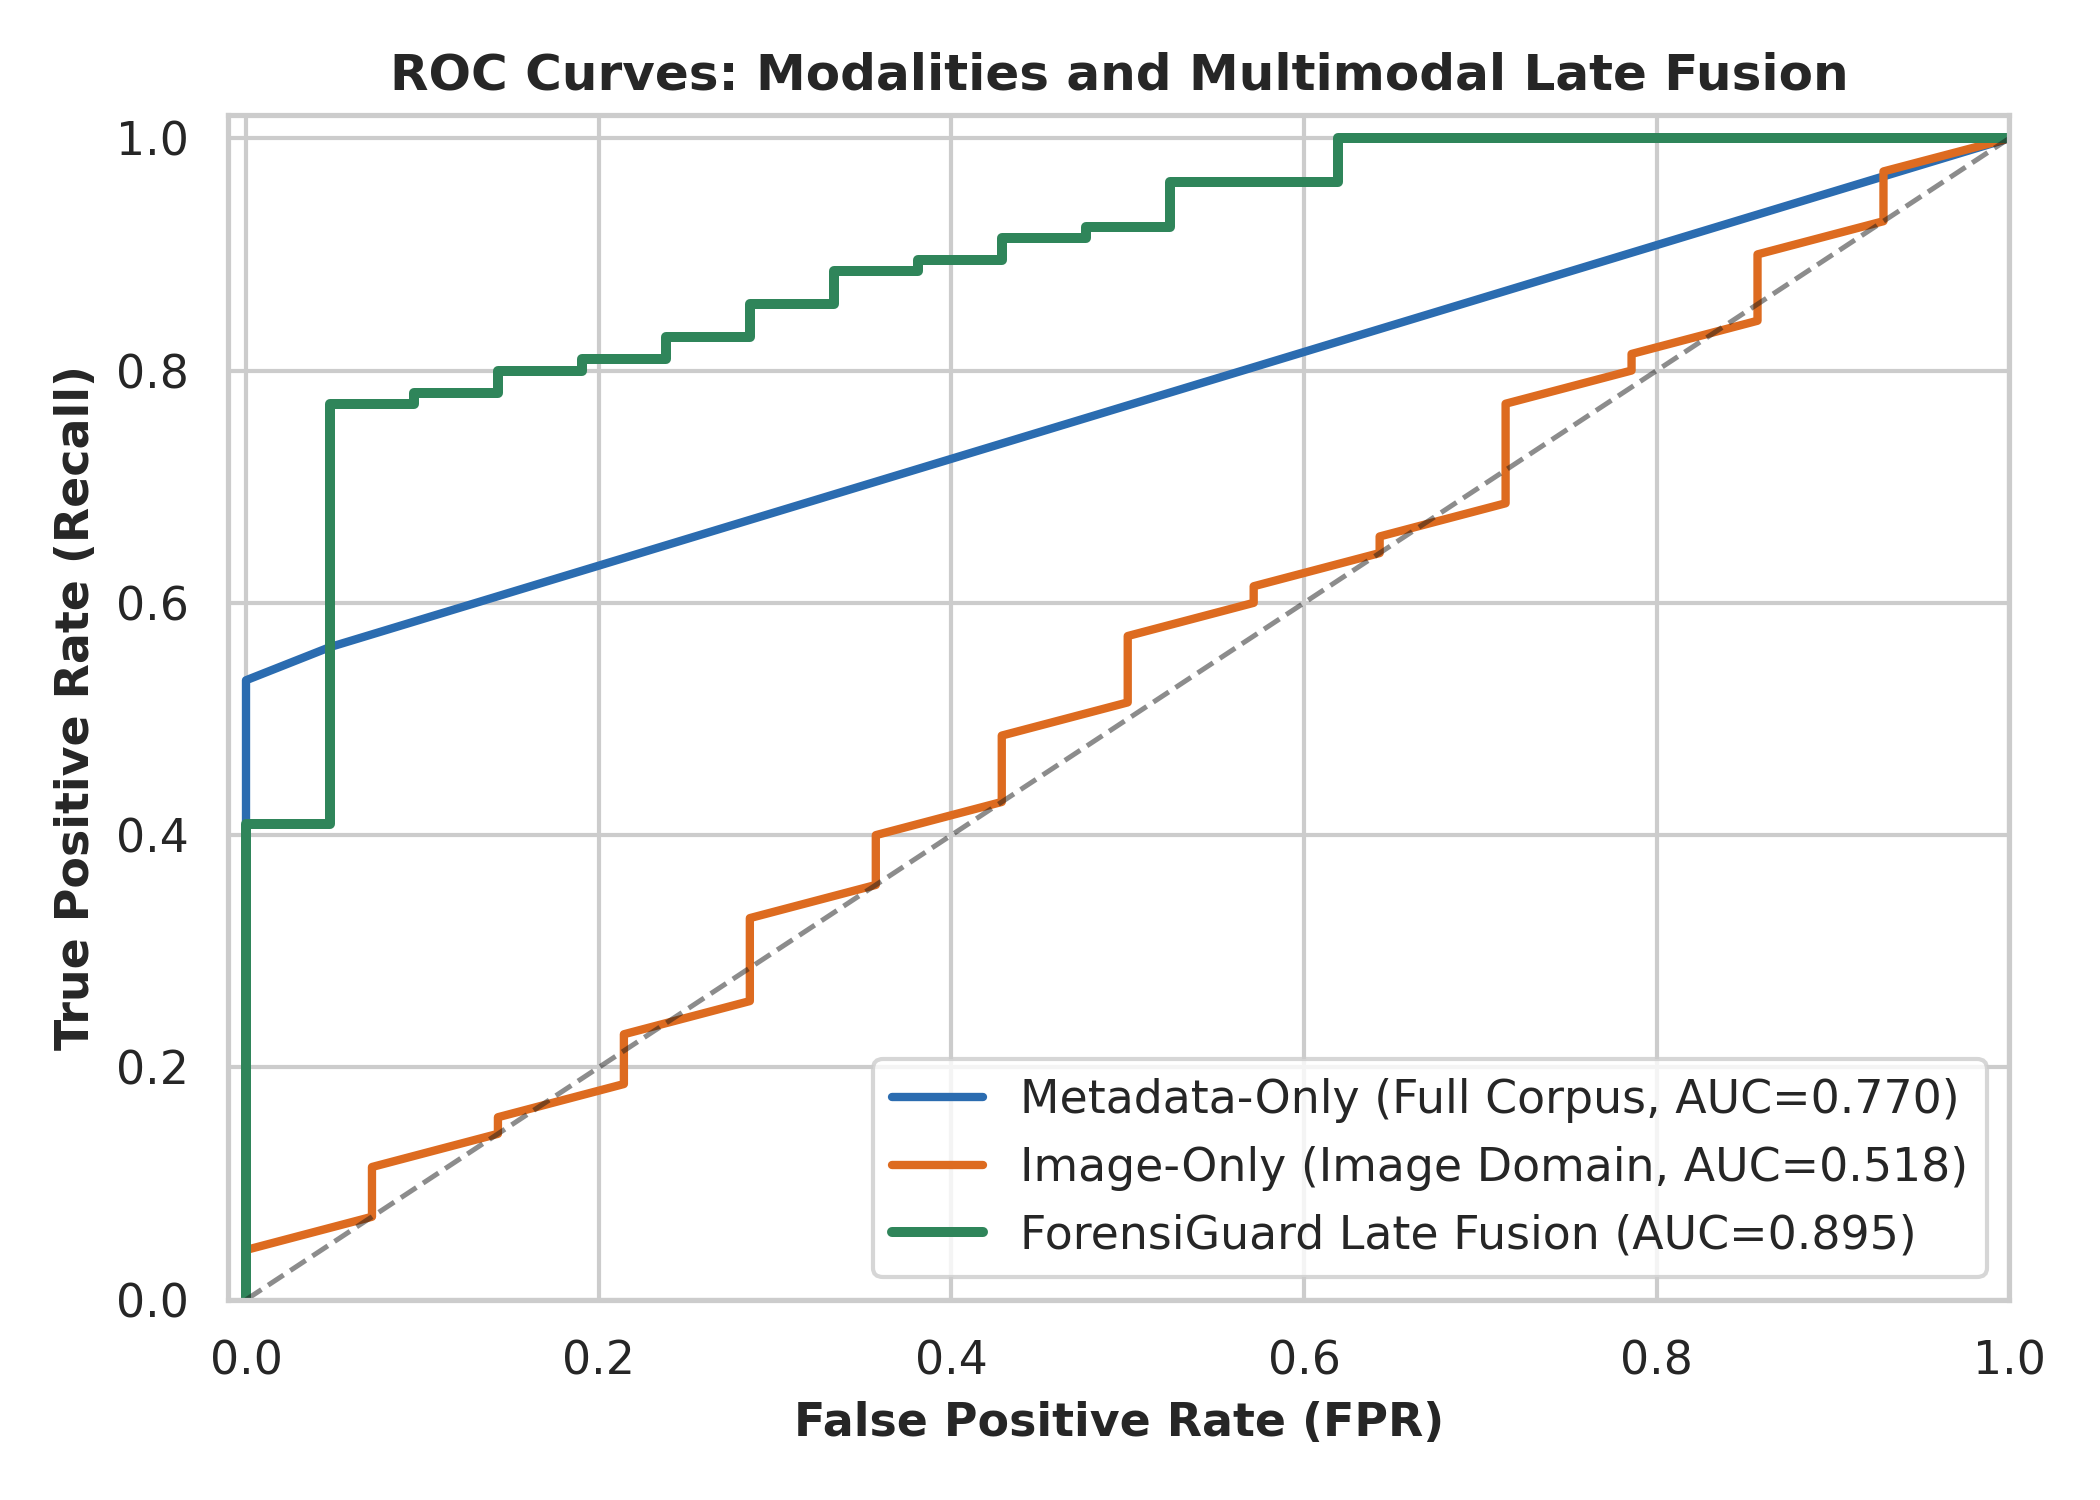
\includegraphics[width=0.92\columnwidth]{figures/fig1_roc_comparison.png}
\caption{Receiver Operating Characteristic (ROC) curves comparing single modalities against ForensiGuard multimodal late fusion on the held-out test split.}
\label{fig:roc}
\end{figure}

\begin{figure}[htbp]
\centering
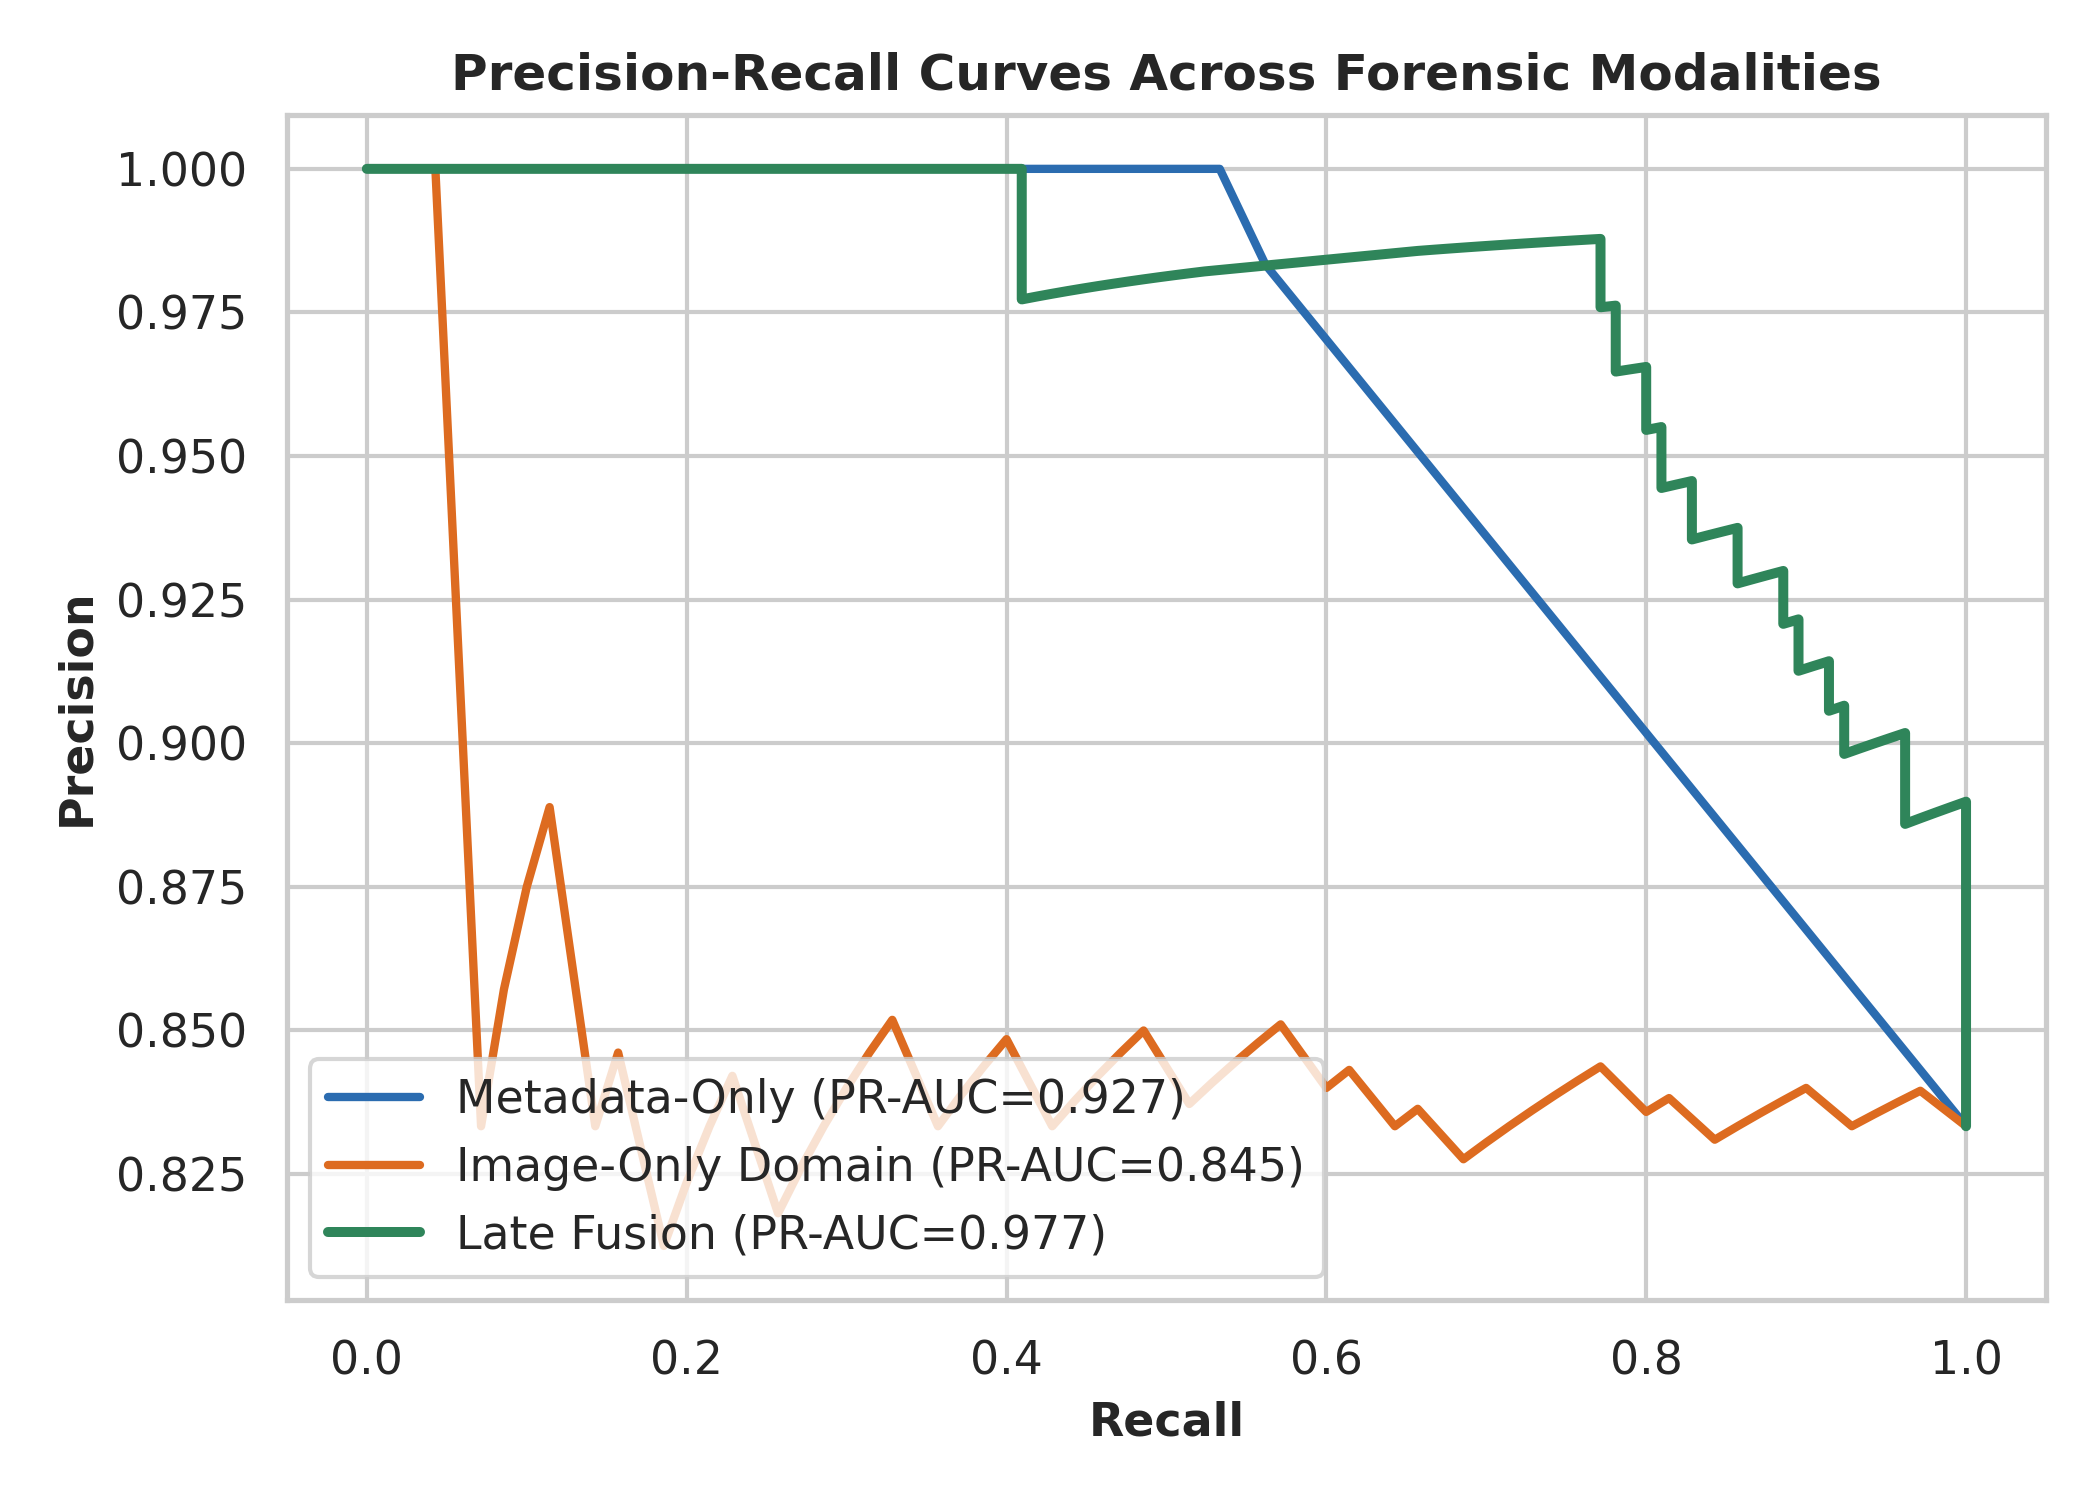
\includegraphics[width=0.92\columnwidth]{figures/fig2_pr_comparison.png}
\caption{Precision-Recall curves showing the continuous discriminative advantage of multimodal late fusion across operating thresholds.}
\label{fig:pr}
\end{figure}

\begin{figure}[htbp]
\centering
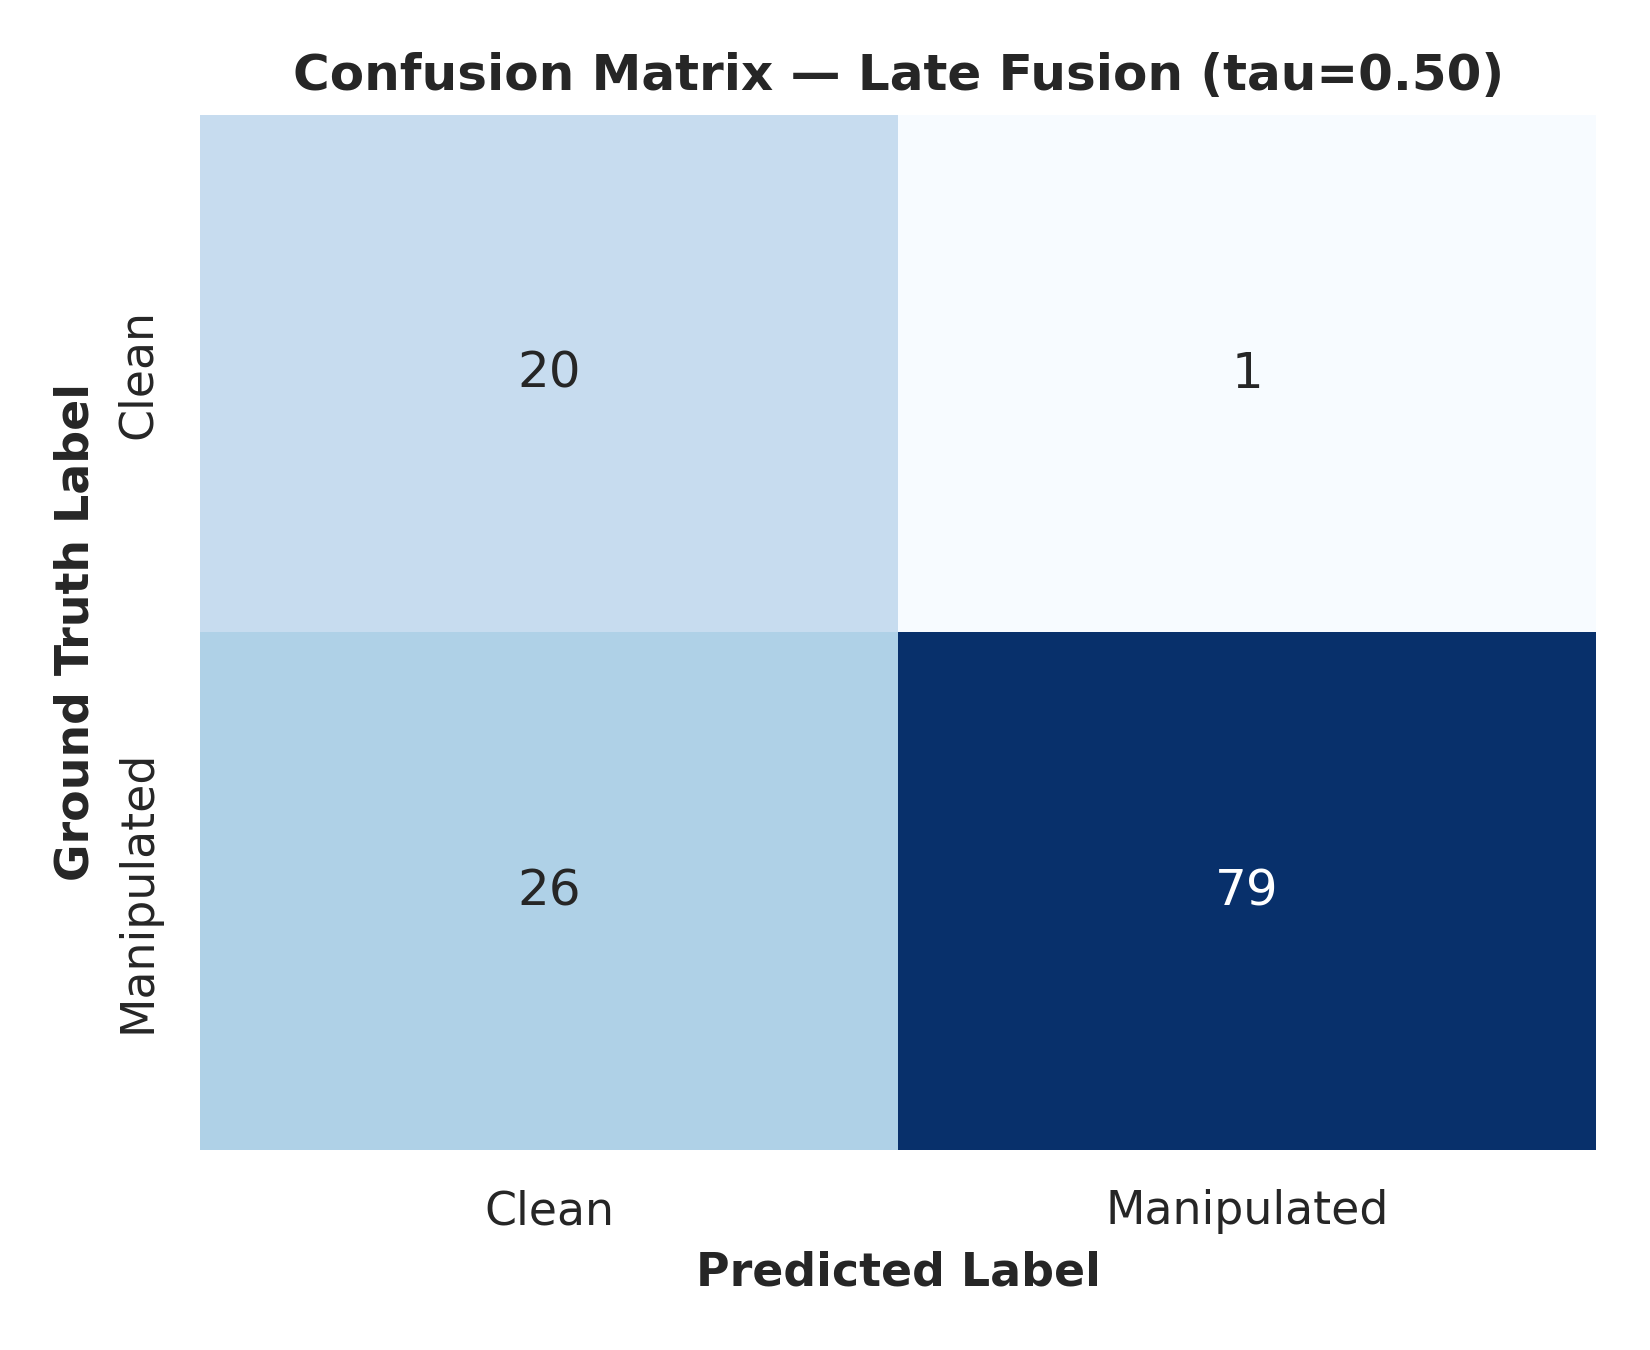
\includegraphics[width=0.72\columnwidth]{figures/fig3_confusion_matrix.png}
\caption{Confusion matrix of ForensiGuard Late Fusion on the held-out test split ($N=126$, $\tau = 0.500$).}
\label{fig:cm}
\end{figure}

\begin{table}[htbp]
\centering
\caption{Ablation Analysis Across Ten Architectural Permutations on Held-Out Test Corpus ($N=126$)}
\label{tab:ablation}
\begin{tabular}{|l|c|c|c|c|c|}
\hline
\textbf{Ablation Variant} & \textbf{Acc.} & \textbf{F1} & \textbf{ROC-AUC} & \textbf{PR-AUC} & \textbf{FPR} \\ \hline
1. Metadata-Only (Base Metadata) & 0.627 & 0.715 & 0.770 & 0.927 & 0.048 \\ \hline
2. Image-Only (Full Corpus) & 0.484 & 0.606 & 0.508 & 0.840 & 0.476 \\ \hline
3. Metadata + Image Model & 0.627 & 0.715 & 0.794 & 0.950 & 0.048 \\ \hline
4. Metadata + Anomaly Score & 0.627 & 0.715 & 0.770 & 0.927 & 0.048 \\ \hline
5. Metadata + Signature Verification & 0.786 & 0.854 & 0.861 & 0.956 & 0.048 \\ \hline
\textbf{6. Full ForensiGuard Late Fusion} & \textbf{0.786} & \textbf{0.854} & \textbf{0.895} & \textbf{0.977} & \textbf{0.048} \\ \hline
7. Full Fusion w/o Image CNN & 0.786 & 0.854 & 0.895 & 0.977 & 0.048 \\ \hline
8. Full Fusion w/o Folder Context & 0.786 & 0.854 & 0.895 & 0.977 & 0.048 \\ \hline
9. Full Fusion w/o Anomaly Scoring & 0.786 & 0.854 & 0.894 & 0.977 & 0.048 \\ \hline
10. Full Fusion w/o Signature Verification & 0.627 & 0.715 & 0.744 & 0.945 & 0.048 \\ \hline
\end{tabular}
\end{table}


\begin{figure}[htbp]
\centering
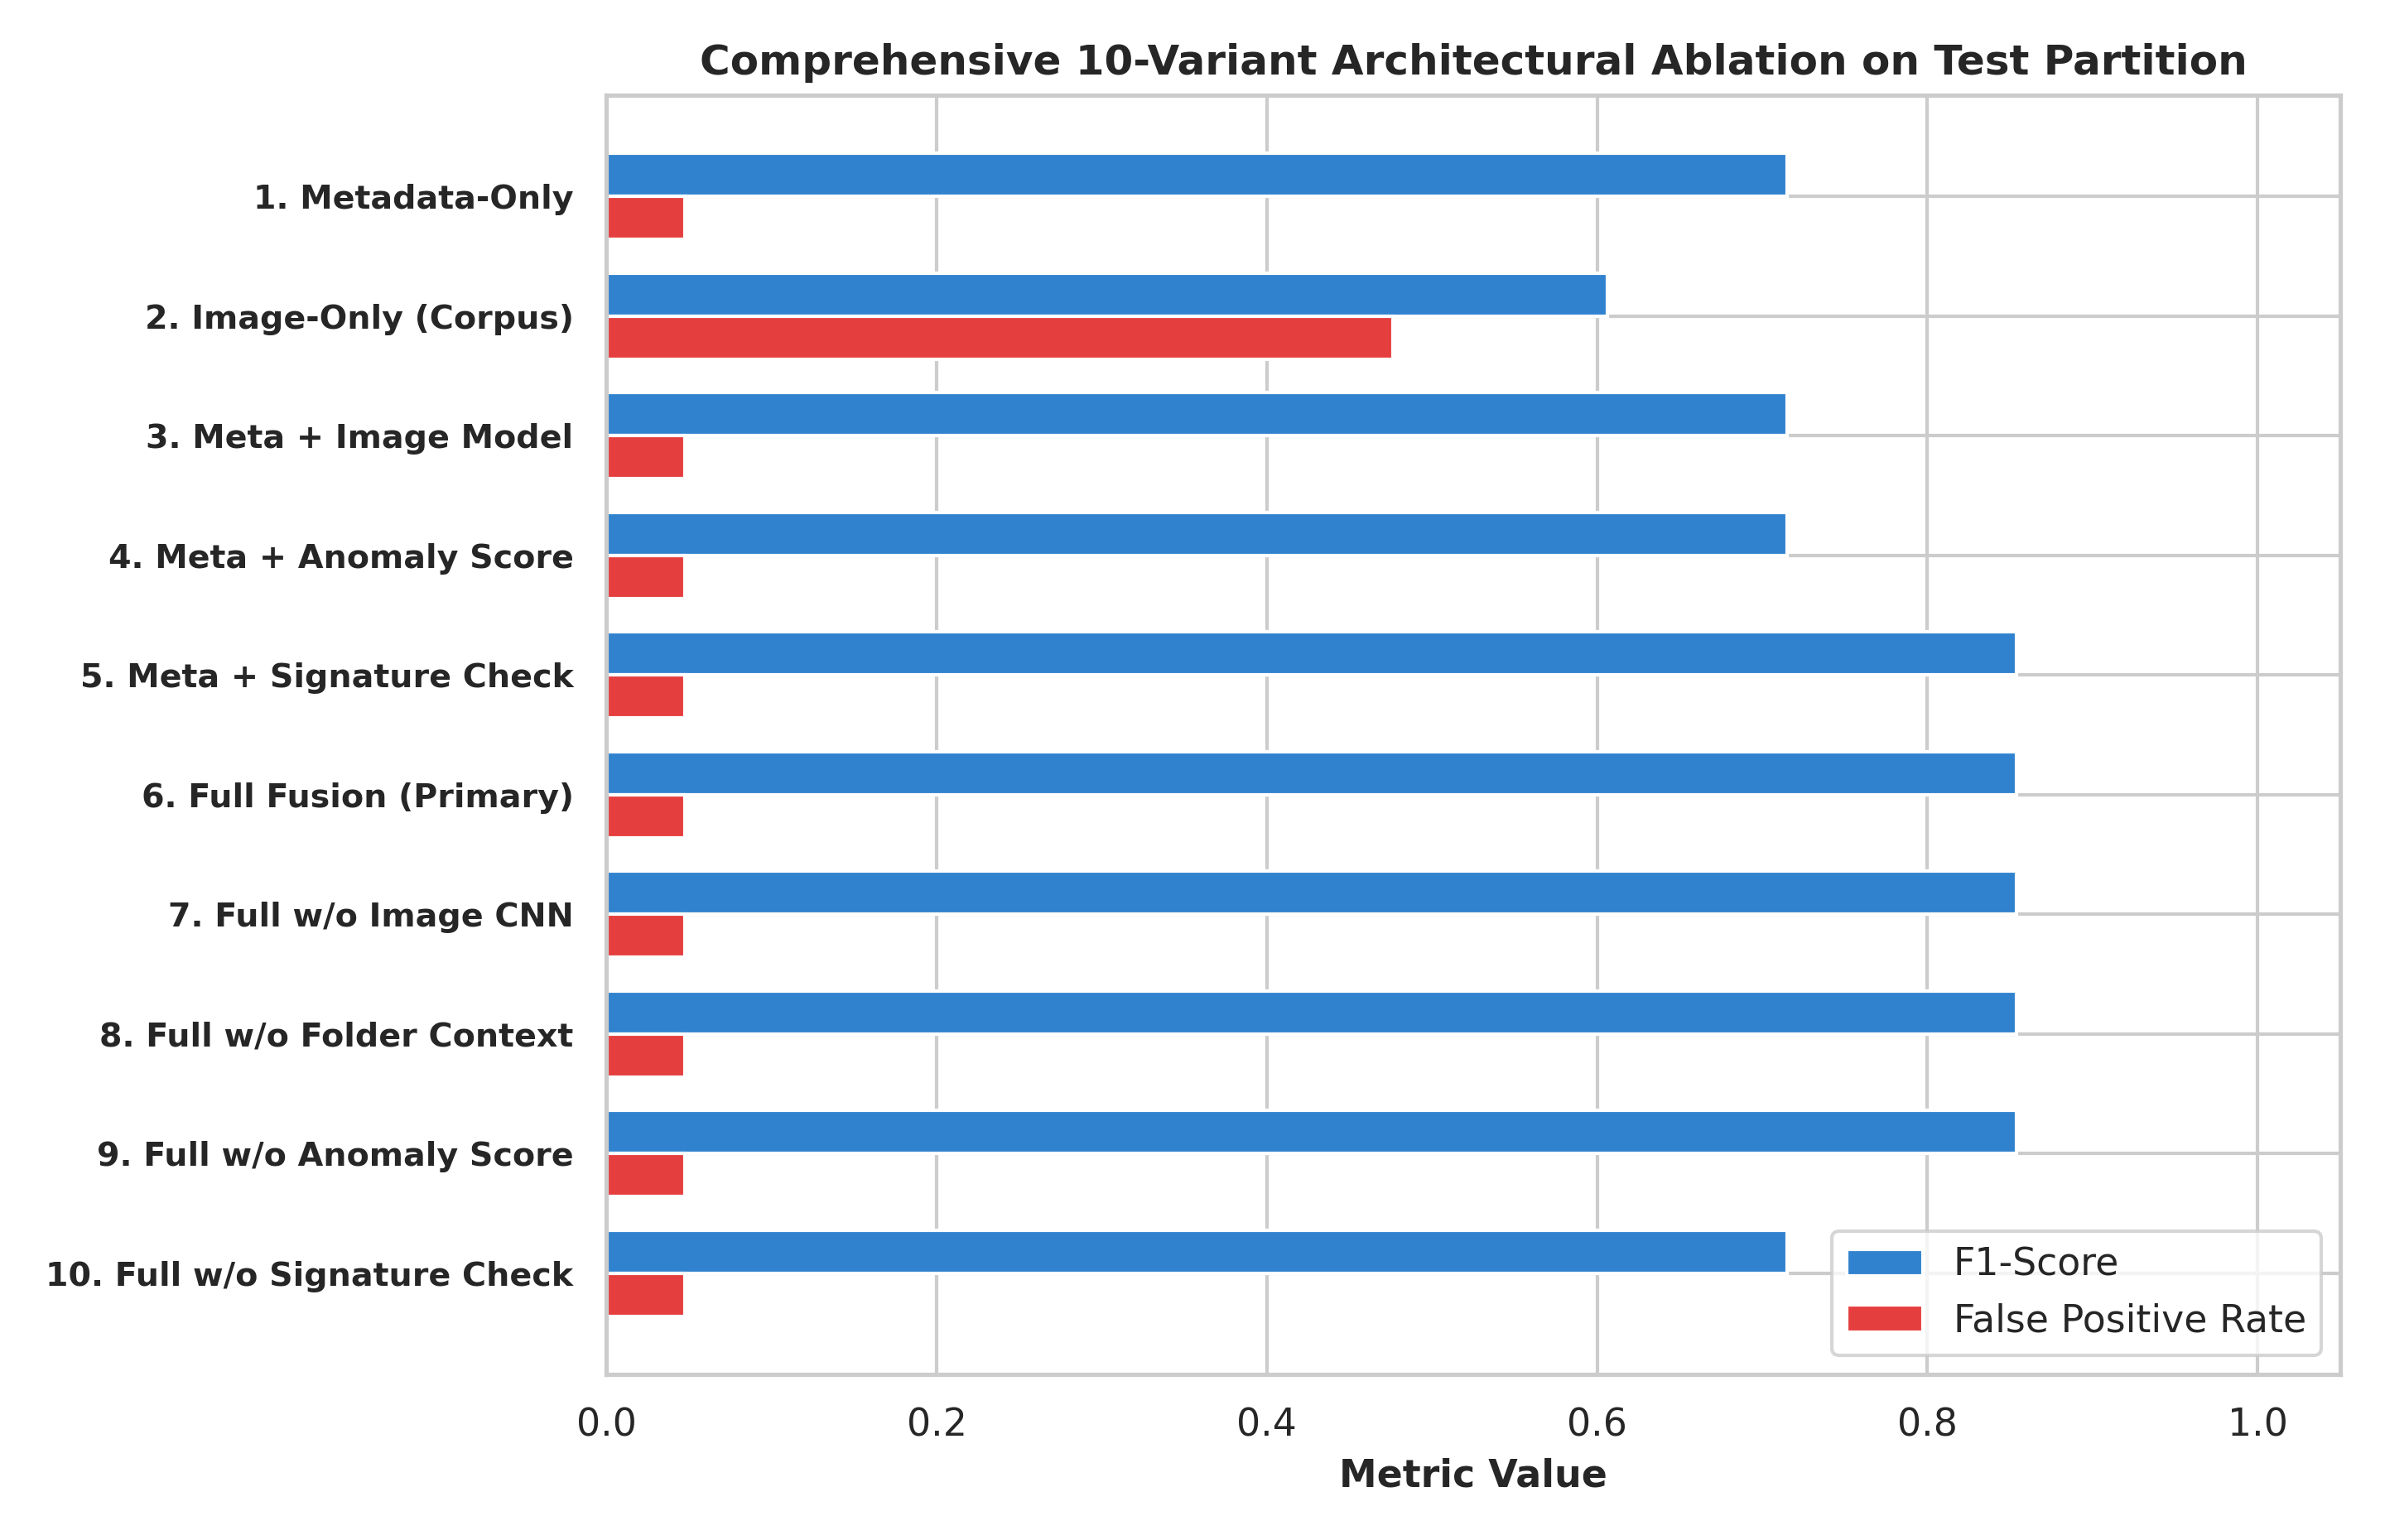
\includegraphics[width=0.95\columnwidth]{figures/fig4_ablation_study.png}
\caption{Ablation analysis illustrating F1-score across ten distinct architectural permutations on the held-out test split.}
\label{fig:ablation}
\end{figure}

\subsection{Component Ablation Studies}
Table~\ref{tab:ablation} and Fig.~\ref{fig:ablation} detail the ten-variant ablation analysis:
\begin{enumerate}
    \item \textbf{The Magic-Byte Discontinuity:} Comparing Variant 1 (Metadata-Only, F1 0.715) to Variant 5 (Metadata + Signature, F1 0.854) reveals that deterministic file signature verification is the single largest driver of discrete F1 improvement (+13.9 percentage points), successfully detecting 21/21 obfuscated files that evade timestamp analysis.
    \item \textbf{Continuous Ranking Optimization:} While Variant 5 and Variant 6 share identical discrete F1 (0.854), Full Late Fusion (Variant 6) achieves higher ROC-AUC (0.895 vs. 0.861) and lower Brier calibration error (0.125 vs. 0.146).
    \item \textbf{CNN Ablation Reality (Variant 7 vs. Variant 6):} Removing the Image CNN (Variant 7) produces identical thresholded Accuracy (0.786), F1 (0.854), Precision (0.988), Recall (0.752), and ranking ROC-AUC (0.895) to Full Late Fusion. Metadata and signature verification completely govern discrete decisions on this corpus. The CNN provides zero thresholded classification or ranking gain; its sole observable contribution is a slight calibration refinement, shifting the Brier score from 0.132 to 0.125.
    \item \textbf{Signature Indispensability (Variant 10):} Omitting signature verification causes F1 to collapse from 0.854 to 0.715 and ROC-AUC from 0.895 to 0.744, proving that cross-modal signature inspection is the essential driver of non-metadata coverage.
\end{enumerate}

\subsection{Attribution Performance}
ForensiGuard's multi-class attribution hierarchy was evaluated across three distinct operational formulations:
\begin{enumerate}
    \item \textit{5-Class Exact Match Accuracy:} \textbf{65.08\%} (82/126 total test artifacts correctly assigned to their exact ground-truth class among Clean, Timestomping, Steganography, File-Type Obfuscation, and Compound).
    \item \textit{Conditional Attribution on Manipulated Artifacts:} \textbf{71.43\%} (75/105 confirmed manipulated artifacts assigned to their true manipulation mechanism, excluding clean files).
    \item \textit{Coarse Binary Attribution:} \textbf{88.89\%} (112/126 artifacts correctly categorized under coarse benign versus manipulated triage).
\end{enumerate}
The confusion matrix reveals two primary misattribution patterns: (i) 28 timestomped files were attributed to Compound due to minor residual noise triggering heuristic stego flags, and (ii) clean files with textured backgrounds occasionally triggered false steganography alerts. File-type obfuscations were attributed with 100\% precision and 100\% recall.

\subsection{Explainability Analysis}
Analysis of five representative test cases illustrates how local TreeSHAP attributions ground triage decisions in physical filesystem evidence:
\begin{itemize}
    \item \textbf{True Positive Coarse Timestomp:} In artifact \texttt{art\_src\_0001} (subtype \textit{coarse\_multiyear}), a 5-year backward jump generated $\Delta_{m,c} = -1.58 \times 10^8$\,s (43,800\,h backdated), contributing $+5.026$ SHAP toward suspicious. Directory deviation ($-20.0\sigma$) added $+0.025$, driving fusion probability to $0.983$.
    \item \textbf{True Positive Subtle Timestomp:} In artifact \texttt{art\_src\_0001} (subtype \textit{subtle\_2h}), a 2.5-hour backward shift ($\Delta_{m,c} = -9,003$\,s) contributed $+5.026$ SHAP, and parent directory outlier status ($-5.14\sigma$) added $+0.025$, resulting in fusion probability $0.983$.
    \item \textbf{False Positive Clean Artifact:} In unaltered artifact \texttt{art\_src\_0092}, synthetic file creation jitter introduced a small delta ($\Delta_{m,c} = -5.00$\,s), contributing $+3.743$ SHAP toward suspicious. This pushed fusion probability to $0.975$, accounting for the single false alarm on the test set.
    \item \textbf{False Negative Steganography:} In pure steganography artifact \texttt{art\_src\_0001} (subtype \textit{high\_payload}), timestamps remained unaltered ($\Delta_{m,c} = -2.73$\,s, SHAP $-4.843$ benign). The metadata model produced a low probability ($0.0037$), resulting in a sub-threshold fusion probability of $0.274$ ($< \tau = 0.500$).
    \item \textbf{True Positive Compound Tampering:} In artifact \texttt{art\_src\_0001} (subtype \textit{stego\_and\_timestomp}), a 30-day timestomp ($\Delta_{m,c} = -2.59 \times 10^6$\,s, SHAP $+5.026$) combined with spatial payload injection yielded fusion probability $0.983$.
\end{itemize}

\subsection{Adaptive-Attack Evaluation}
In our adaptive attack stress test, an adversary shifted timestamps by 3.5 hours, bounded the shift within directory variance, preserved microsecond fractions ($0.482910$\,s), and updated creation time synchronously to eliminate chronology inversion ($t_m \ge t_c$).
Under these conditions:
\begin{itemize}
    \item The isolated metadata XGBoost model recorded a \textbf{0.0\% detection rate} (mean probability $0.0039$).
    \item The Isolation Forest anomaly scorer detected slight distributional shift ($S_{\text{anom}} = 0.596$), raising fusion probability to $0.216$.
    \item However, because $0.216 < \tau = 0.500$, the late-fusion model also recorded a \textbf{0.0\% detection rate}.
\end{itemize}
This result empirically demonstrates that static filesystem timestamps cannot counter an adversary who preserves all temporal invariants, proving the theoretical necessity of correlating operating system event logs (e.g., Windows Event ID 4616: ``System time was changed'').

\subsection{Error Analysis}
On the held-out test split, ForensiGuard produced 1 False Positive and 26 False Negatives. The single False Positive arose from microsecond file creation jitter. The 26 False Negatives were subtle steganographic images whose timestamps and headers remained unaltered; because spatial LSB alterations in uncompressed carriers produce imperceptible noise, they evaded both metadata and CNN detection.

\section{Threats to Validity and Limitations}
\begin{enumerate}
    \item \textbf{Synthetic Benchmark Scope and Clustered Provenance:} \texttt{ForensiGuard-Bench-v1} provides verified ground truth under strictly controlled generation parameters. However, the evaluation partition comprises 126 artifacts derived from only 21 independent source groups ($N_{\text{sources}}=21$). Clustered dependencies widen statistical uncertainty intervals, and high benchmark accuracy does not imply off-the-shelf production readiness across complex, multi-terabyte enterprise storage or in-the-wild incident response.
    \item \textbf{Steganalysis Constraints and CNN Ablation Reality:} Consistent with the ablation results, the lightweight residual CNN yields no discrete classification or ranking gain over fusion-without-CNN on the test set, contributing solely a minor calibration adjustment. Detecting subtle spatial LSB payloads on uncompressed carriers without container shortcuts remains an open research problem requiring extensive domain-adapted pretraining.
    \item \textbf{Filesystem Granularity:} Legacy filesystems (e.g., FAT32) natively truncate timestamps to 2-second increments; zero subseconds on FAT32 must not be interpreted as timestomping.
    \item \textbf{Adaptive Evasion Limits:} Static metadata analysis is fundamentally limited against adversaries who preserve relative temporal invariants.
    \item \textbf{Evidentiary Demarcation and FRE 901:} Under Federal Rule of Evidence 901 (Authenticating or Identifying Evidence), machine-learning classification scores, anomaly probabilities, and SHAP attributions are heuristic triage leads designed to prioritize manual inspection. They do not establish evidence authenticity, chain of custody, or legal admissibility in judicial proceedings.
\end{enumerate}

\section{Conclusion and Future Work}
ForensiGuard provides an explainable, multimodal machine-learning framework for defensive forensic triage. By combining filesystem metadata, spatial noise residuals, and binary file signatures through grouped out-of-fold late fusion, the system achieves an Accuracy of 78.57\%, an F1-score of 0.854, an ROC-AUC of 0.895, and an operational False Positive Rate of 4.76\% on a benchmark free of container shortcuts and source leakage. Our adaptive attack evaluation highlights the limits of static metadata inspection. Future work will integrate sequential operating system audit logs (Windows Event IDs 1102 and 4616) via sequence transformers to close the gap against invariant-preserving temporal adversaries.

\section*{Acknowledgment}
The authors thank the Department of Data Science and Computer Applications at Manipal Institute of Technology, Manipal Academy of Higher Education (MAHE), for providing the computing infrastructure and experimental facilities.

\bibliographystyle{IEEEtran}
\bibliography{references}

\end{document}
